\chapter{Implementação do Ambiente de DWing}
\label{estudo de caso}

\section{Arquitetura da Implementação}

Para a implementação do ambiente do DWing para métricas de código-fonte, foi definida a arquitetura tal como se mostra Figura \ref{arquitetura}.


\begin{figure}[ht!]
\centering
\includegraphics[keepaspectratio=false,scale=0.20]{figuras/arquitetura-dwing.eps}
\caption{Arquitetura do Ambiente de Dwing para Métricas de Código-Fonte}
\label{arquitetura}
\end{figure}
\FloatBarrier

Para selecionar as ferramentas, que implementarão cada um dos componentes do ambiente DWing, estabeleceram-se critérios gerais de seleção tal como pode ser visto na Tabela \ref{seleção}.


	\begin{table}[!ht]
	\begin{center}
	 \begin{tabular}{|l|l|}
		\hline
		Identificador & Critério 
		\\ \hline
		CG01 & A ferramenta deve possuir código aberto.  
		\\ \hline
		CG02 & A ferramenta deve ter documentação disponível em inglês e português.      
		\\ \hline
		CG03 & A ferramenta deve possuir uma comunidade ativa em seu uso.
		\\ \hline
		CG04 & A ferramenta deve possuir releases estáveis.    
		\\ \hline
		\end{tabular}
		\caption{Critérios Gerais de escolha das ferramentas}
		\label{seleção}
		\end{center}
		\end{table}	


\section{Ferramenta de Análise Estática de Código-Fonte}

Além dos critérios gerais estabelecidos, para escolha da ferramenta de análise estática de código-fonte, que são as fontes externas de coleta, estabeleceram-se os critérios específicos para seleção de ferramentas de análise estática de código fonte (CAE) apresentados na Tabela \ref{specific}


	\begin{table}[!ht]
	\begin{center}
	 \begin{tabular}{|l|p{10cm}|}
		\hline
		Identificador & Critério 
		\\ \hline
		CAE01 & A ferramenta deve prover as métricas de código-fonte para as linguagens de programação, tal como especificado na Tabela \ref{metrics}.
		\\ \hline
		CAE02 & A ferramenta deve possuir saída de dados em arquivo em alguns dos seguintes formatos: JSON, XML, TXT, CSV.      
		\\ \hline
		CAE03 & A ferramenta deve ser mutiplataforma.
		\\ \hline
		\end{tabular}
		\caption{Critérios Específicos para Ferramenta de Análise Estática de Código-Fonte}
		\label{specific}
		\end{center}
		\end{table}	

Após a realização de uma busca por ferramentas, foram encontradas o SonarQube~\footnote{Disponível em \url{http://www.sonarqube.org/}} e Analizo~\footnote{Disponível em \url{http:/http://analizo.org/}} cujas principais características de ambas são apresentadas na Tabela \ref{dados-ferramentas-estatica}
\begin{savenotes}
\begin{table}[!ht]
\centering
\begin{tabular}{|p{5cm}|p{4.5cm}|p{5cm}|}
\hline

Característica 

&

\begin{center}

\includegraphics[keepaspectratio=false,scale=0.48]{figuras/analizo.eps} 
\end{center}


&



\begin{center}
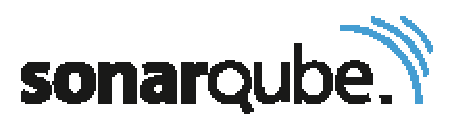
\includegraphics[keepaspectratio=false,scale=0.48]{figuras/sonarqube.eps} 
\end{center}





   
\\ \hline


%--------------------------
Linguagens com Suporte  & C, C++, Java & C, C++, Java, PHP,Scala, Python, Delphi, Pascal, Flex, ActionScript, Javascript, Groovy~\footnote{O SonarQube oferece suporte comercial a outras linguagens, contudo foram listadas apenas que tem suporte por meio de \textit{plugins} de código-aberto} \\ \hline
Licença  & GNU GPL3 & GNU LGPL3  \\ \hline



%--------------------------
Formato de Saída das Métricas  & CSV, YAML & JSON, XML, CSV \\ \hline

%--------------------------
Plataforma  &Windows, Linux, Mac OS X e Servidores de Aplicação Java & Debian e Ubuntu                                                                                              \\ \hline

%--------------------------
Integração com outras ferramentas & Mezuro,Kalibro & Jenkins, Hudson, Mantis, JIRA, Crowd e entre outros \\ \hline

%--------------------------
\multirow{4}{5cm}{Números do Repositório Oficial no GitHub em 14/11/2013}
& \textit{Commits:} 7532 & \textit{Commits:} 639\\ \cline{2-3} 

&\textit{Branches:} 16 & \textit{Branches:} 1  \\ \cline{2-3} 
& Contribuidores: 18 & Contribuidores: 7  \\ \cline{2-3} 
& \textit{Releases:} 36  & \textit{Releases:} 27

 \\ \hline

%--------------------------
Número de Casos Abertos no \textit{Issue Tracker} em 14/11/2013 & 552  & 26 
\\ \hline

%--------------------------
Sistema de Controle de Versões & Git & Git \\ \hline

%--------------------------
Idioma com Suporte & Inglês & Inglês, Português, Japonês, Italiano, Chinês, Francês, Grego e Espanhol \\ \hline

%------------------------
Idioma da Documentação & Inglês & Inglês

\\ \hline
%-----------------------
Última Versão Estável em 14/11/2013 & 1.17.0 & 4.0  

\\ \hline
 %-----------------------
Data de Lançamento da Última Versão Estável & 31 de Janeiro de 2013 & 4 de Novembro de 2013

\\ \hline
\end{tabular}
\caption{Caractrísticas do SonarQube e do Analizo}
\label{dados-ferramentas-estatica}
\end{table}
\FloatBarrier
\end{savenotes}

Tendo as características gerais de cada ferramenta levantadas, foram comparadas (SonarQube e Analizo) quanto aos critérios gerais e aos critérios específicos para ferramentas de análise estática, tal como se mostra na Tabela \ref{compare}



\section{Ferramenta de Extração, Transformação e Carga (ETL)}

\section{Projeto do \textit{Data Warehouse}}

\section{Ferramenta de Apoio as Consultas OLAP e Visualização de Dados}
% Critérios de Selecção de Ferramentas

% \section{SonarQube}
% O SonarQube~\footnote{Toda a documentação e \textit{downloads} estão disponíveis
% em \url{http://www.sonarqube.org/}}, anteriormente conhecido como Sonar, é uma 
% ferramenta que realiza coleta de dados do código-fonte. Em sua documentação, 
% são citados sete eixos de controle de qualidade cobertos na ferramenta: 

% \newlist{qualityindex}{enumerate}{4}
% \setlist[qualityindex]{ label* = \arabic* -}

% \begin{qualityindex}
% \item Duplicação de Código
% \item Detecção de Complexidade de Código
% \item Padrão de Codificação
% \item Testes Unitários
% \item Arquitetura e Projeto
% \item Potenciais Defeitos
% \item Comentários
% \end{qualityindex}

% %--------------------------------------------%
% \subsection{Escolha do SonarQube}
% O SonarQube foi escolhido como ferramenta para extração de dados do código-fonte
%  devido as seguintes características:
% \begin{description}
  
% \item [Ferramenta Livre:] O SonarQube é uma ferramenta livre que está 
% licenciada sob a GNU LPGL 3, que é uma das licenças de software livre.

% \item [Suporte a várias Linguagens de Programação:]  É realizada coleta em 
% mais de 20 linguagens de programação, como por exemplo, Java, C\#, Python, 
% C++, .Net, PHP e entre outras.

% \item [Multiplataforma:] Há suporte para os sistemas operacionais Windows, 
% Linux, Mac OS e há também para servidores de aplicação Java, como por exemplo,
% o Apache Tomcat. 

% \item [Integração com Ferramentas de Integração Contínua:] é possível realizar
% a integração com ferramentas de integração contínua, como por exemplo, 
% Jenkins. Assim a cada versão bem sucedida de construção do código-fonte, é 
% possível aferir a qualidade do código.

% \item [Persistência em Base de Dados:] toda a coleta de dados é persistida em 
% uma base de dados. Há suporte para as principais ferramentas de bancos de 
% dados utilizadas no mercado: MySQL, PostgreSQL e Oracle.

% \item [Interface Amigável:] Diferentemente de outras ferramentas disponíveis 
% no mercado, o SonarQube tem interface web, ou seja, é possível visualização 
% das métricas do código-fonte seja realizada em navegador a escolha do usuário.
% É possível ainda visualizar todo o código-fonte analisado.

% \item [Integração com Ferramentas de Gestão de Defeitos:] É possível integrar 
% com ferramentas de gestão de defeitos, tais como Mantis e JIRA.

% \item [Suporte a Muti produtos:] Há suporte para visualização de métricas de 
%  mais um Produto.

% \item [Suporte a Multi-Idiomas:] Há suporte para Inglês, Japonês, Russo, 
% Francês, Italiano, Espanhol e Português.

% \item [Diversidade de Plugins:] O SonarQube permite a 
% extensão de funcionalidades por meio de plugins, sendo que há uma variedade de 
% plugins para mais diversas necessidades disponíveis para \textit{download}. 
% Cabe ressaltar que alguns são gratuitos e outros tem licença comercial.

% \item [Presença de Web Service:] Há um Web Service que extrai as métricas 
% disponíveis para diversos formatos, tais como JSON, XML e CSV.

% \end{description}


% %--------------------------------------------%


% \subsection {Limitações Observadas}
% Após uma análise ostensiva na ferramenta, concluiu-se que o SonarQube apresenta 
% as seguintes limitações:

% \begin{description}

% \item [Ausência de Visão Consolidada de Métricas:]  A maior parte das métricas
% que SonarQube estão apenas no âmbito de Classes ou Pacotes.

% \item [Impossibilidade Definição de Múltiplos Intervalos:]  O sonarQube não 
% permite a configuração de múltiplos intervalos. É definido apenas, um 
% intervalo de alerta (amarelo) e um intervalo de atenção (vermelho).

% \item [Ausência de Avaliações Qualitativas:] As métricas não trazem nenhuma 
% avaliação qualitativa associada, ou seja, sem o conhecimento específico do 
% significado de cada métrica, a interpretação dos valores obtidos não é 
% representativo nem elucidativo sobre a qualidade do código.

% \item [Métricas como Violações:] O SonarQube utiliza para coletar dados de 
% código-fonte, em algumas linguagens de programação, coletores que são 
% identificadores de padrões de codificação. Isso quer dizer que algumas métricas 
% não são apresentadas com valor absoluto, apenas são indicadas como violações à 
% regras estabelecidas pelos padrões. 

% \end{description}




% \section{Pentaho}

% O Pentaho é um software de código aberto para inteligência empresarial, 
% desenvolvido em Java pela Pentaho Corporation, que apresenta soluções cobrindo 
% as áreas de ETL, \textit{reporting}, OLAP e mineração de dados 
% (\textit{data-mining}). 


 
